\begin{answer}

we can use the three neurons in the hidden layer to form linear decision boundaries that resemble the sides of a triangle, effectively separating the two classes in the dataset.

The idea is to configure each neuron in the hidden layer $(h_1, h_2, h_3)$ to activate (output 1) for data points on one side of its corresponding decision boundary and to not activate (output 0) for points on the other side. 

By simple inspection, we can come up with the following decision boundary
\begin{equation}
    h1 = -x_1 - x_2 + 4 > 0 
\end{equation}
\begin{equation}
    h2 = - x_1 + 0.5 > 0
\end{equation}
\begin{equation}
    h3 = -x_2 + 0.5 > 0 
\end{equation}

And for activation, area inside triangle have sum equals to 0, otherwise greater than 0. So we use the following weight
\begin{equation}
    h1 + h2 + h3 > 0
\end{equation}

\begin{figure}[H]
    \centering
    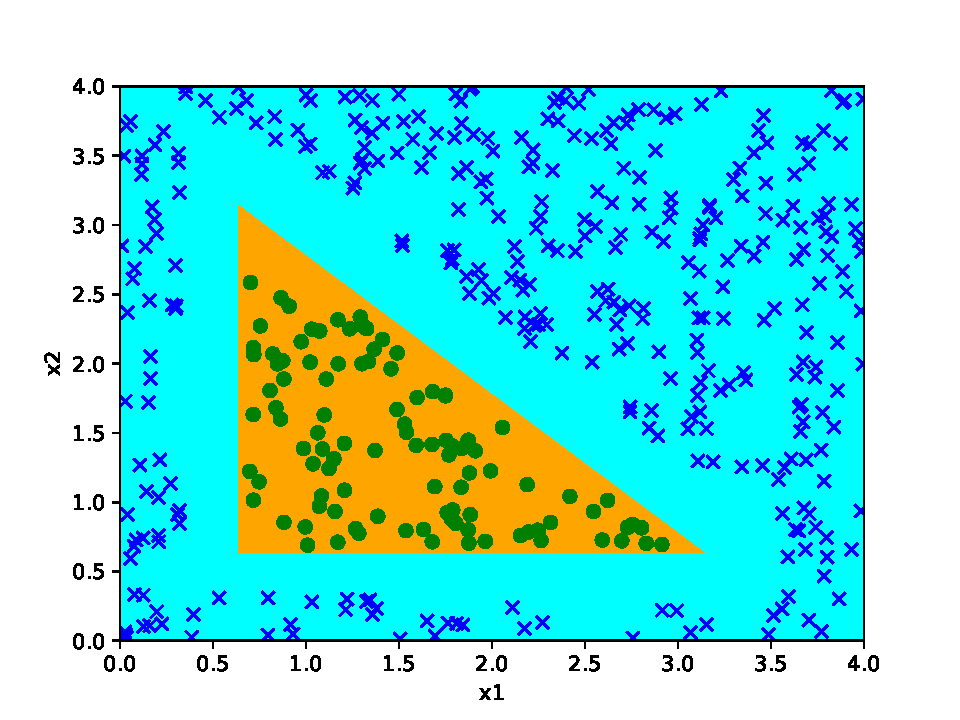
\includegraphics[width=0.5\linewidth]{step_weights.pdf}
    \caption{ps3::q5::(b)}
    \label{fig:enter-label}
\end{figure}
\end{answer}
